%4.2.tex

\ref{chp:4_1}で述べたLLVMのRISC-Vバックエンドでの命令生成のための命令定義クラスについて,ベクトル拡張付きRISC-Vのベクトル命令のための命令フィールドと命令の定義を行った.

図\ref{fig:MIQSInst_class}
に定義した命令フィールド定義クラスと命令定義のためのクラスの継承関係を示す.

\begin{figure}[tb]
    \centering
    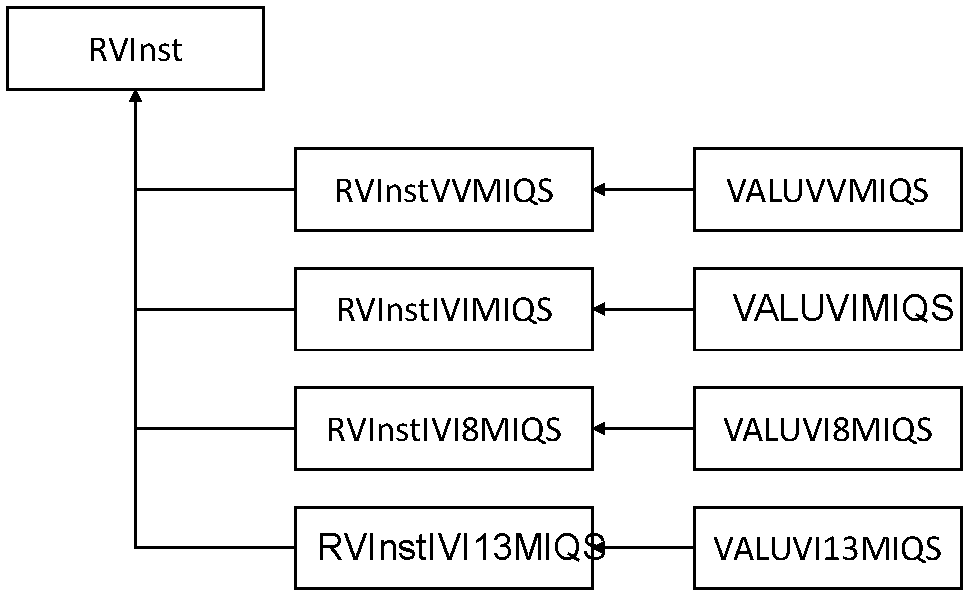
\includegraphics[scale=0.6]{image/MIQSInst_class.pdf}
    \caption{定義したクラスの継承関係}
    \label{fig:MIQSInst_class}
\end{figure}

本研究ではベクトル拡張付きRISC-Vの命令のうち,ベクトル演算命令のプレディケートレジスタを用いない命令を実装した.
プレディケートレジスタを用いない命令はオペランドで用いるレジスタや命令の種類が類似しているため,プレディケートレジスタを用いている命令より比較的容易に実装が可能である.

実装した命令とそのフォーマットを図\ref{fig:jissou_inst_format}
にまとめる.

\begin{figure}[tb]
    \centering
    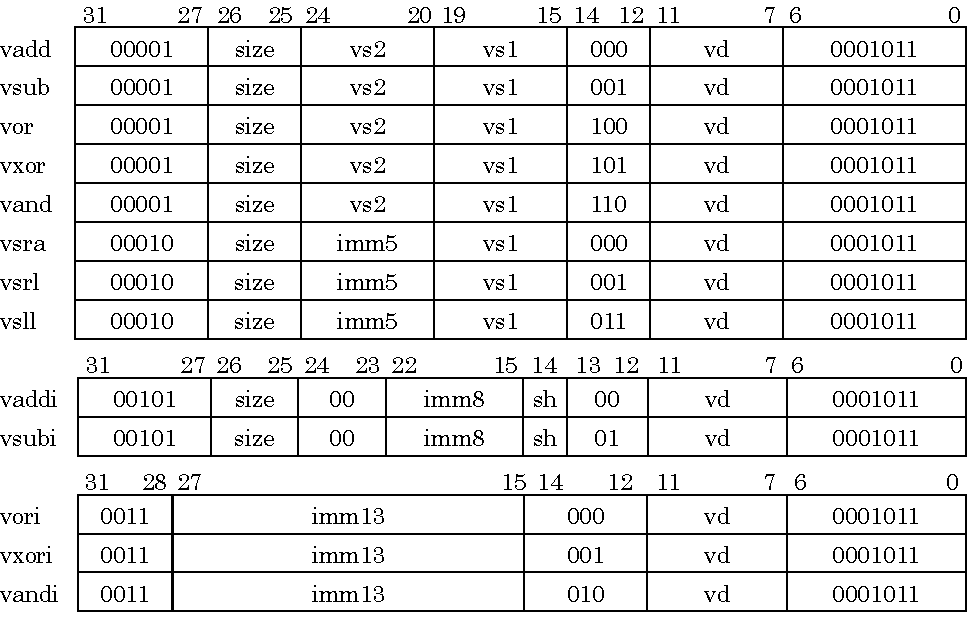
\includegraphics[scale=0.8]{image/jissou_inst_format.pdf}
    \caption{実装した命令}
    \label{fig:jissou_inst_format}
\end{figure}

図\ref{fig:jissou_inst_format}
vaddなどの命令フォーマットの26-25ビットにて指定されているsizeはベクトル要素のサイズを指定するためのフィールドであり,この値に応じたサフィックスが命令の末尾に追加されるものである.本研究では整数要素の処理の場合のみを想定し,このsizeの値は32ビットサイズを表すために'0b10'で固定している.また,即値を用いた算術演算命令であるvaddi,vsubiの命令フィールドのうち14ビットのshは24-20ビットで指定した即値を8ビットシフトするかを決定するためのフィールドである.このフィールドが0である場合はシフトを行わず,1であるときは8ビットのシフトを行う.このshの値はvaddi等の命令のオペランドにて指定を行うが,本研究ではシフトを行わない0で値を固定している.

実際に定義した命令フォーマットクラスの一覧を図\ref{fig:jissou_inst_format_class}
に示す.RVInstVVMIQSはvadd,vsub,vor,vxor,vandのための命令フォーマットで.RVInstIVIMIQSは5ビットの即値を用いるvsra,vsrl,vsll用の命令フォーマット,RVInstIVI8MIQSは8ビットの即値を用いるvaddi,vsubi用の命令フォーマット,RVInstIVI13MIQSは13ビットの即値を用いるvori,vxori,vandi用の命令フォーマットの定義である.

\begin{figure}[tb]
    \centering
    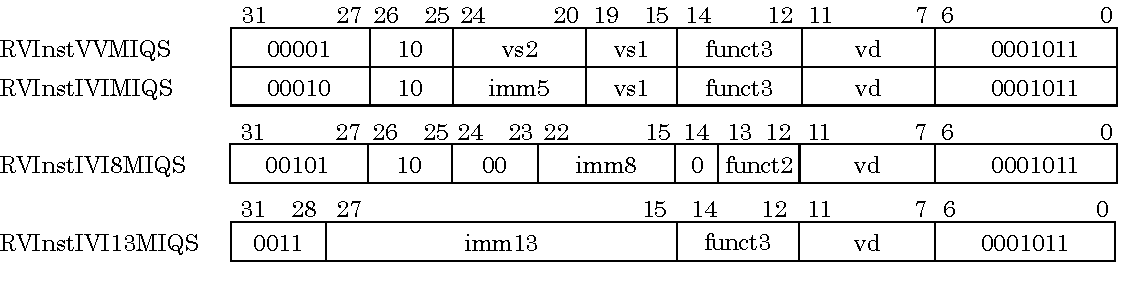
\includegraphics[scale=0.8]{image/jissou_inst_format_class.pdf}
    \caption{実装した命令フォーマットクラス}
    \label{fig:jissou_inst_format_class}
\end{figure}

また,実際のTableGenによる定義の例としてRVInstVVMIQSの定義を図\ref{fig:RVInstVVMIQS}
に示す.図\ref{fig:jissou_inst_format_class}
で示したフォーマットとなるように命令フィールドInstのどのフィールドにどの値が格納されるかを指定する.

\begin{figure}[tb]
    \centering
    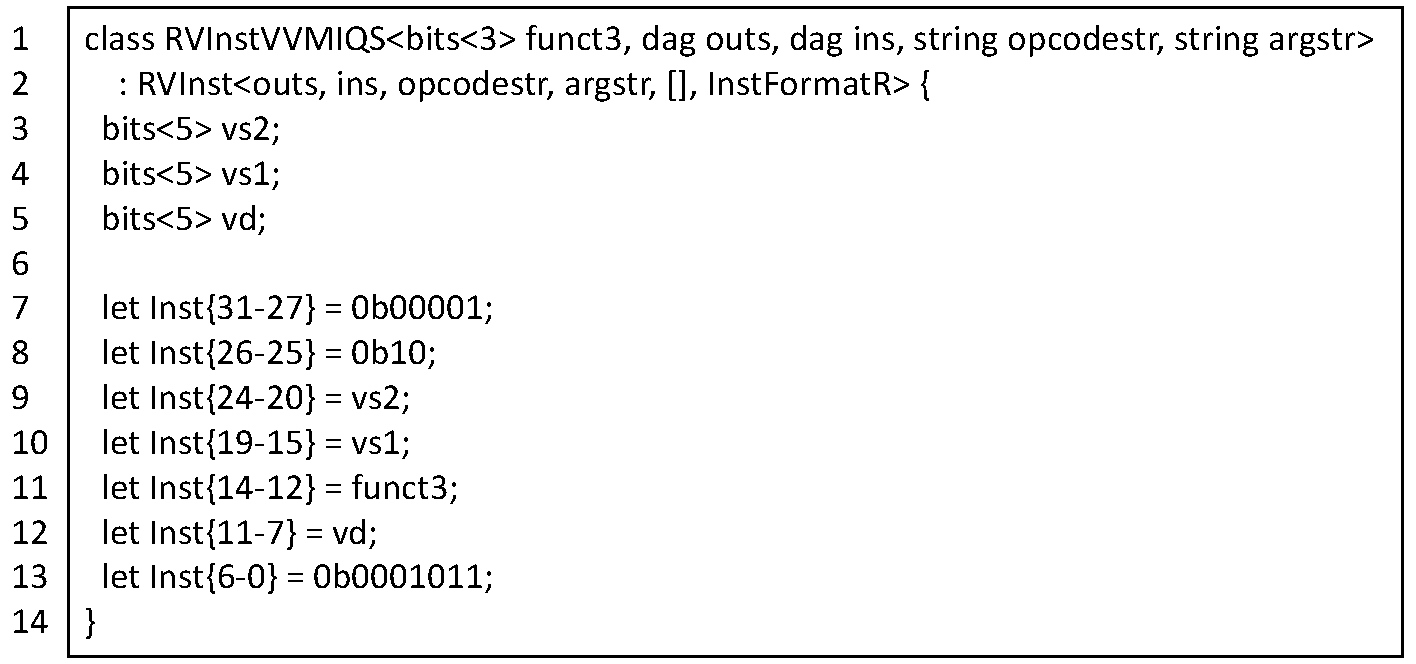
\includegraphics[scale=0.6]{image/RVInstVVMIQS_v2.pdf}
    \caption{TableGenによるRVInstVVMIQSの定義}
    \label{fig:RVInstVVMIQS}
\end{figure}

命令の定義を図\ref{fig:Inst_def}
に示す.
図\ref{fig:Inst_def}
のALUVVMIQSはベクトル同士の演算を行うための命令の定義用に定義の繰り返しを防ぐためのクラスである.ALUVVMIQSでは出力レジスタと入力レジスタの指定を行う.このクラスを定義することで例えば``vadd.w vd vs1 vs2''と``vsub.w vd vs1 vs2''のようにオペランドが同じ命令の定義を行う場合,ALUVVMIQSをインスタンス化する際に入出力レジスタの定義を繰り返しを防ぐことができる.

命令のインスタンス化も図\ref{fig:Inst_def}
で行っている.ベクトル算術・論理演算命令のインスタンス化を行っている.引数では命令の文字列と命令選択のための値を指定している.

\begin{figure}[tb]
    \centering
    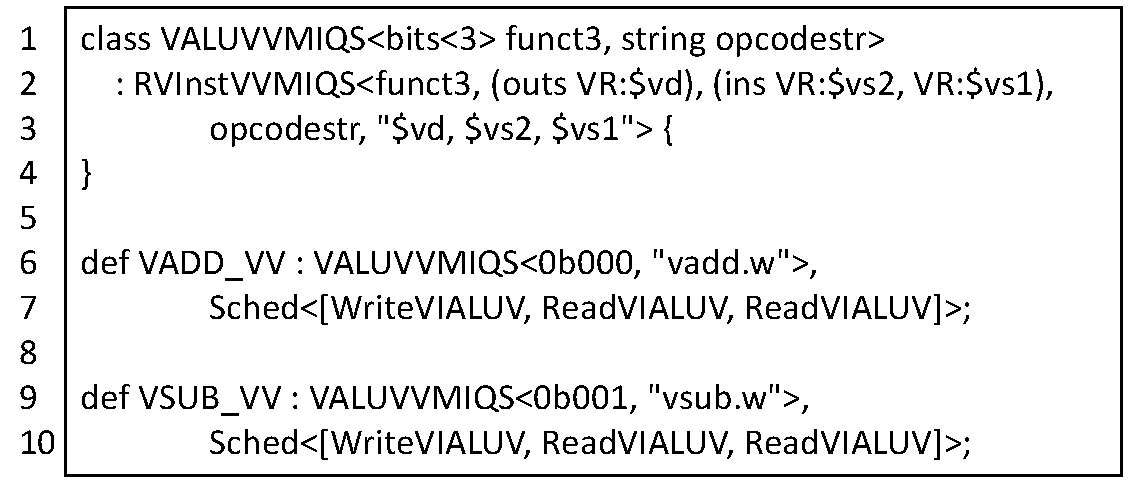
\includegraphics[scale=0.6]{image/Instruction_define.pdf}
    \caption{命令の定義}
    \label{fig:Inst_def}
\end{figure}

TableGenによる命令の定義は以上の様に行われ,残りの命令フォーマットや命令についても同様に定義を行った.
